\documentclass{tikzposter} %Options for format can be included here
%\usepackage{listings}

 % Title, Author, Institute


\makeatletter
\def\TP@titlegraphictotitledistance{-10cm}
\settitle{ \centering \vbox{
\@titlegraphic \\ [\TP@titlegraphictotitledistance] 
\centering
\color{titlefgcolor} {\bfseries \Huge \sc \@title \par}
\vspace*{1em}
{\huge \@author \par} \vspace*{1em} {\LARGE \@institute}
}}
\makeatother

\setlength{\columnsep}{2cm}
%
\title{\parbox{\linewidth}{\centering Convenient analysis of numerous \\
distance sampling data sets in R}}
\author{Eric Rexstad, David L. Miller, Lindesay Scott-Hayward}
\institute{Centre for Research into Ecological and Environmental Modelling, University of St. Andrews} % St. Andrews Scotland KY16 9LZ}
\titlegraphic{
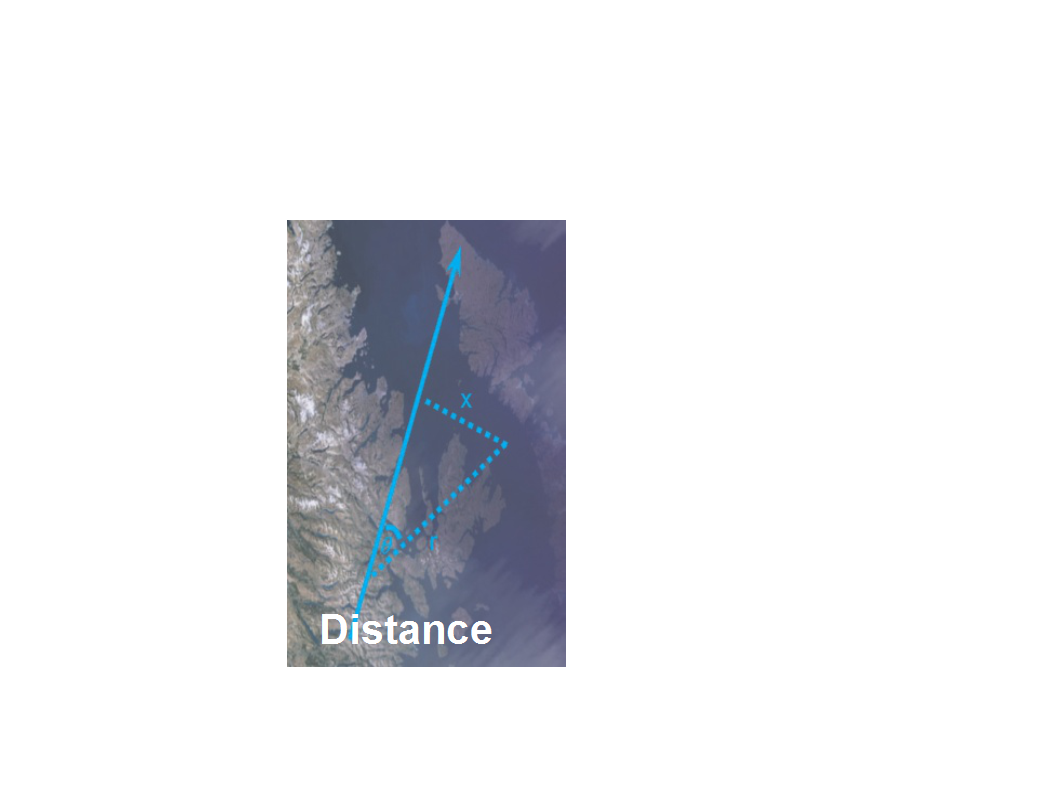
\includegraphics[scale=4.0]{distancelogo.png}
\hfill 
\vspace{30pt} %\\
\includegraphics[scale=0.35]{foundation-vertical-colour.png}
}



 %Choose Layout
\usetheme{Board} % Autumn, Desert, Envelope, Wave, Board, Basic, Rays, Simple
\usepackage [sfdefault]{cabin}
\usepackage[T1]{fontenc}
\usepackage{multirow}

\definecolor{almond}{rgb}{0.94, 0.87, 0.8}
\definecolor{lightcornflowerblue}{rgb}{0.6, 0.81, 0.93}
\definecolor{sunglow}{rgb}{1.0, 0.8, 0.2}

\begin{document}
%\lstset{language=R}

 % Title block with title, author, logo, etc.
\maketitle

\begin{columns}

\column{0.5}
 \block{Challenges of analysis of archival data}{
 \begin{itemize}
  \item As questions about animal populations become more complex, so do the data and analytical requirements,
  \item Few of us analyse data from a single survey of a single species, 
  \item It is increasingly common to use archival data (defined as data collected for one purpose but used for another purpose) to assess spatial and/or temporal change in animal density.
 \end{itemize}
 
 We describe a generic set of tools to permit thoughtful analysis of archival data.  This involves exploratory data analysis (EDA), collaborative decisions about analysis steps, reproducible audit trail of analysis steps.  As described in an ISEC2010 plenary talk by Jeff Laake, reproducible research is a desirable goal of any analysis project.  However with multiple interested parties, reproducibility climbs the priority list. 
}

\column{0.5}
 % First column - third block
\block{Purpose of analysis}{
Produce seasonal density surfaces of seabirds combining aerial and shipboard surveys for 41 species groupings.  

Large volume of data collected (>2000000 records), requirement to produce density surfaces for species $\times$ season combinations.  Detection functions to adjust for incomplete detectability created for each survey platform (planes and boats).  

Visual inspection of the distribution of detection distances was necessary before analysis because:
\begin{itemize}
\item detections for some season/platform combination were sparse,
\item geographic coverage for some season/platform combinations was poor, or
\item distribution of detection distances for some combinations was not conducive to detection function modelling.
\end{itemize}

}

\end{columns}
 
 \begin{columns}


\column{0.25}

\block{Familiarity with data}{
\begin{itemize}
\item If analyst = data collector, this step happens by default. 
\item Otherwise, exploratory data analysis is more elaborate.
\item If there are other collaborators, exploratory analysis may be protracted.
\begin{itemize}
\item Analysis decisions may involve not only data provider and analysts but other parties who commissioned the analysis.
\item This is made simpler through the use of \textsl{analysis notebook} that can be shared among investigators.
\item Audit trail is produced to permit tracing of evidence used in analysis decisions.
\end{itemize}
\end{itemize}
}

\block{Inventory phase of EDA}{
Archival data are high dimensional.  There are requisites necessary for robust estimates of animal density derived from distance sampling methods.  These requisites include adequacy both of survey \textbf{\textsl{effort}} and \textbf{\textsl{sightings}} mutually in the dimensions of
\begin{itemize}
\item species,
\item time (year or season), and
\item geographical area.
\end{itemize}
\begin{itemize}
\item In a perfect world, there would be a balanced design in which there were sufficient data for all combinations of species $\times$ season $\times$ region, but data are seldom perfect,
\item Some combinations are likely to be missing or under-represented,
\item With insufficient effort or detections, estimation of animal density will be fruitless at best and misleading at worst.
\end{itemize}

%\vspace*{6cm}
}

\block{}{
\vspace*{2cm}
\includegraphics[scale=0.5]{isec2014.jpg}\\
\coloredbox[bgcolor=sunglow]{University of St. Andrews is a charity registered in Scotland: SCO13532}
}


\column{0.75}

\begin{subcolumns}
\subcolumn{0.56} \block{Example EDA results}{
We developed R Markdown code to perform the exploratory analyses and prepare a notebook page for each of the 41 species groupings of interest.

\coloredbox [bgcolor=almond]{\includegraphics[scale=1.3] a}} 
\note[targetoffsetx=-13.2cm, targetoffsety=6.9cm, angle=90, radius=0, rotate=25]{{\small \raggedright Spatial effort in U.K. waters by season}}
\note[targetoffsetx=-21cm, targetoffsety=-11cm, angle=20, rotate=25]{{\small \raggedright Distribution of perpendicular distances season $\times$ platform}}
\note[targetoffsetx=+7cm, targetoffsety=-2cm, angle=20, rotate=-25]{{\small \raggedright Sightings by season $\times$ platform}}
\note[targetoffsetx=+6cm, targetoffsety=-13cm, angle=20, rotate=-25]{{\small \raggedright Distribution of observed cluster sizes}}


\block{Fitting detection functions using Distance}{
Distance is an uncluttered interface to the MRDS R package for fitting detection functions.  Data that contain rudimentary fields (region label, region area, transect length, perpendicular distance) are amenable to analysis without extensive data preparation.  

The multi-species seabird database was organised such that fitted detection probabilities can be extracted, following the EDA with code such as 
\coloredbox [bgcolor=lightcornflowerblue] {
	\texttt{library(Distance) \\
		pr.detect <- numeric(0, length=3) \\
		for (species.name \%in\% c("FULMAR","GANNET","SCOTER")) \{ \\
		  \hspace{1cm} pr.detect[i] <- ds(data[species==species.name,], \\        
		                 \hspace{2cm}     truncation="0\%", key="hr", \\
		                 \hspace{2cm}     adjust=0)\$dht\$individuals\$average.p \\
		\}  
	}
}
	
If there is a balanced design (adequate effort and sightings for all combinations of strata defined by \texttt{Region.Label}), the "split-apply-combine" strategy can be employed to conduct wholesale analyses.

\coloredbox [bgcolor=lightcornflowerblue] {
\texttt{models <- dlply(data,.(Region.Label),ds) \\
sapply(models, plot)  \# view fitted models \\
count.adjustment <- sapply(models, function(x) x\$dht\$individuals\$average.p) \# p\_i for this stratum
}
}
}

\subcolumn{0.44}

\block{"Industrial-scale" analysis}{
	\begin{itemize}
	\item Facilitated by use of detection function fitting routines in Distance R package (Miller 2014),
	\item We visually assessed perpendicular distance distributions for all species $\times$ season $\times$ platform combinations,
		\begin{itemize}
		\item The distribution of the perpendicular distances was placed into one of three categories:
			\begin{itemize}
			\item distribution of data did not support fitting of a detection function,
				\begin{itemize}
				\item remove that species $\times$ season $\times$ platform combination, or
				\item treat as strip transect,
				\end{itemize}
			\item fitting of data supported after truncation,
			\item fitting of detection function to untruncated data.
			\end{itemize}
		\end{itemize}
	\item After categorisation, it was straightforward to perform "bespoke" modelling for the 164 species $\times$ season $\times$ platform combinations. 
	\end{itemize}
}

\block  {Web-based analysis}{

The next step in collaborative analysis between data provider, analyst and funding agent is placing the entire enterprise on the web.

\coloredbox [bgcolor=lightcornflowerblue] {
Some of this can be done using the Shiny interface for R.  Jeff Laake, National Marine Fisheries Service in the U.S. is developing such an interface for components of Distance.

\begin{center}
	\includegraphics[scale=0.8]{shiny.png}
\end{center}
}
}

\block [bodywidthscale=0.75, titlewidthscale=0.75]{To learn more}{
\begin{tabular}{p{13cm} c}
Distance package (CRAN) & \raisebox{-.5\height}{\includegraphics[scale=0.5]{qrcodecrandistance.png}} \\ 
\raggedright Distance Shiny app  (jlaake.shinyapps.io/Distance) & \raisebox{-.5\height}{\includegraphics[scale=0.5]{qrcodeshiny.png}} \\ 
\raggedright distancesampling.org \newline (New Distance website) & \raisebox{-.5\height}{\includegraphics[scale=0.5]{qrcodedistancesamplingorg}} \\
\end{tabular} 
}
\end{subcolumns}

\end{columns}
\end{document}